\documentclass{article}


\usepackage{amsmath, amsthm, amssymb, amsfonts}
\usepackage[makeroom]{cancel}
\usepackage{xcolor}
\usepackage{graphicx}
\usepackage{geometry}
\usepackage[american, RPvoltages]{circuitikz}

\usepackage{IEEEtrantools}

\usepackage{hyperref}
\usepackage[utf8]{inputenc}
\usepackage[english]{babel}

\usepackage{ragged2e}

\usepackage{tikz}

\usepackage{siunitx}


\geometry{
    textheight=9in,
    textwidth=7.5in,
    top=1in,
    headheight=12pt,
    headsep=25pt,
    footskip=30pt
}

\newcommand{\smallsignal}[2]{\lowercase{#1}_{\lowercase{#2}}}
\newcommand{\equationname}{Equation}

\newcommand{\cancelRed}[1]{\textcolor{red}{\cancel{\textcolor{black}{#1}}}}
\newcommand{\cancelToOne}[1]{\textcolor{red}{\cancelto{1}{\textcolor{black}{#1}}}}
\newcommand{\cancelToZero}[1]{\textcolor{red}{\cancelto{0}{\textcolor{black}{#1}}}}
\newcommand{\cancelToApproxZero}[1]{\textcolor{red}{\cancelto{\approx 0}{\textcolor{black}{#1}}}}


\newcommand\eqnarraycomment[2][4.5cm]{\parbox[t]{#1}{\RaggedRight #2}}

\DeclareMathOperator{\sign}{sgn}

% center, y0, y1
\newcommand{\drawposregion}[3]{
	\draw[color=black, fill=black!20]  
	  		plot ({#1 + 0.5 + 0.25*cos((3.14159*((#3 - #2)*\x + #2) r)}, {(#3-#2)*\x+#2})
	  		-- ({#1 - 0.5 - 0.25*cos(( 3.14159 * #3 ) r) }, #3)
	  		plot ({#1 - 0.5 - 0.25*cos(-3.14159*(#3 - (#3-#2)*\x) r)}, {#3 - (#3-#2)*\x})
	  		-- ({#1 + 0.5 + 0.25*cos((3.14159*#2 ) r)}, #2);
}

% x0, x1, y0, y1
\newcommand{\drawsquare}[4]{
	\draw (#1, #3)
		-- (#1, #4)
		-- (#2, #4)
		-- (#2, #3);

	\draw[dashed] (#1, #4+0.2) -- (#1, -0.2);
	\draw[dashed] (#2, #4+0.2) -- (#2, -0.2);
}

\begin{document}

% ------------------------------------------------------------------------------
% Cover Page and ToC
% ------------------------------------------------------------------------------

\title{\textbf{\uppercase{Passive Rectifier Impedance}}}
\date{}
\author{\textbf{Eric Ponce} \\
		Massachusetts Institute of Technology}

\maketitle

% \tableofcontents

% ------------------------------------------------------------------------------

\section{Introduction}

This paper discusses and proves some concepts regarding the ac-side impedance of a passive rectifier feeding various types of loads.

The basic model is shown below:

\begin{figure}[htbp]
\center
\begin{circuitikz}
	% ac positive-half-cycle forward current
	\draw (0, -2)
		to[vsourcesin, v=$V_L$] 	++(0, 2)
		to[vsourcesin, v=$v_p$] 	++(0, 2) 
		to[short]					++(2, 0)
		to[short]					++(0,-1)
		to[short, -*, i=$i_{AC}$]	++(2, 0)  % (4, 0.5)
		to[D*] 						++(0, 2); % (4, 3.0)
	% ac positive-half-cycle return current
	\draw (6, -3)
		to[D*] 	++(0, 2);
	% ac negative-half-cycle forward current
	\draw (0, -2)
		to[short] 		++(2, 0)
		to[short] 		++(0, 1)
		to[short, -*] 	++(4, 0)
		to[short] 		++(0, 2)
		to[D*] 			++(0, 2); % (6, 3)
	% ac negative-half-cycle return current
	\draw (4, -3)
		to[D*] 			++(0, 2)
		to[short] 		++(0, 2);
	% ac side voltage
	\draw (3, 1)
		to[open, v=$v_{AC}$] ++(0, -2);
	% dc side
	\draw (4, 3)
		to[short]			 			++(2, 0)
		to[short, i=$i_{DC}$] 			++(2, 0)
		to[generic, l=Load, v=$v_{DC}$] ++(0, -6)
		to[short] 						++(-4, 0);
\end{circuitikz}
\caption{ac-side Impedance Test Circuit.}
\end{figure}

\section{Small Signal Impedance for Continuous Conduction and Linear Loads}

Let $v_{AC}$ be defined by the following time series and fourier series:
\begin{IEEEeqnarray}{rCl}
	v_{AC}(t) &=& V_L\cos(2\pi f_L t) + v_p \cos(2\pi f_P t + \phi_P) \\
	v_{AC}[f] &=& \begin{cases}
					\frac{V_L}{2} \quad & \mathrm{for} \, f=\pm f_L \\
					\frac{v_p e^{j\phi_P}}{2} \quad & \mathrm{for} \, f=\pm f_P
				\end{cases}
\end{IEEEeqnarray} 

Let $m(t)$ be a modulating or mixing signal that is 1 during the positive half cycle and -1 during the negative half-cycle such that:
\begin{IEEEeqnarray}{rCl}
	v_{DC}(t) = v_{AC}(t) \cdot m(t), \label{eq:mixing_step1}\\
	i_{AC}(t) = i_{DC}(t) \cdot m(t). \label{eq:mixing_step2}
\end{IEEEeqnarray}
\textbf{This implicitly assumes that the full-wave rectifier is continuously conducting.}

\subsection{Mixing Signal Derivation}
There are are many ways to derive the perturbed mixing signal, and then to compute its fourier series.
Here we present one that uses double fourier analysis along with a \textbf{small signal pproximation}.

\subsubsection{Double Fourier Integral Approach}
In a non-commutated continuous conduction case, the mixing signal can be defined as
\begin{equation}
	m(t) = \sign\left(v_{AC}(t)\right).
\end{equation}

It can be rewritten the mixing function as a paramteric equation of two functions $x(t)$ and $y(t)$
\begin{IEEEeqnarray}{rCl}
m(t) &=& \sign\left(v_{AC}(t)\right) \nonumber\\
	 &=& \sign\left(V_L\cos(x(t)) + v_p\cos(y(t))\right),
\end{IEEEeqnarray}
where $x(t) = 2\pi f_L t$ and $y(t) = 2\pi f_P t + \phi_P$.

This modulation may be visualized as a set of unit cells that repeat in both directions forever.
Onto this space composed of unit cells we can superimpose the solution trajectory to arrive at
the square wave we expect. 
The solution trajectory is found by substituting the inverse of $x(t)$ into $y(t)$:
\begin{IEEEeqnarray}{rCl}
	t &=& \frac{x}{2\pi f_L} \nonumber\\
	y &=& \frac{f_P}{f_L} x + \phi_p
\end{IEEEeqnarray}

The bounds of the shaded region of the unit cell are found by solving for the zero-crossing
\begin{IEEEeqnarray}{rCl}
	0 &=& v_{AC}(t) \nonumber\\
	0 &=& V_L\cos(x) + v_p \cos(y) \nonumber\\
	x &=& 2 n \pi \pm \arccos (-\frac{v_p}{V_L} \cos y) \quad \forall \, n \in \mathbb{Z} 
\end{IEEEeqnarray}

The unit cell is shown in \figurename ~\ref{fig:double_fourier_unit_cell} and the process by which it maps to $m(x,y)$ is shown in \figurename ~\ref{fig:double_fourier_mapping}
\begin{figure}[htbp]
    \center
	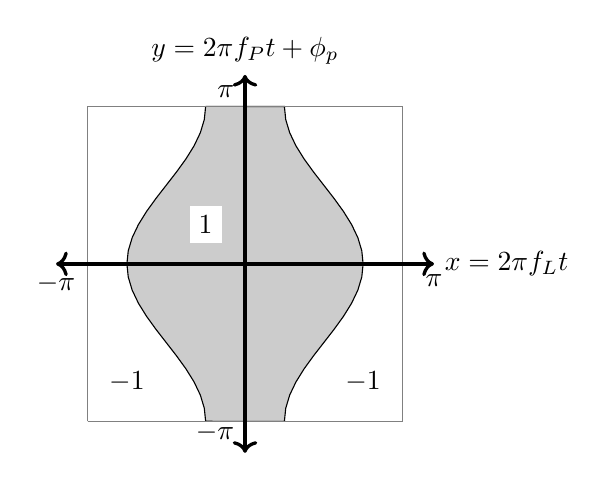
\begin{tikzpicture}[domain=0:1, scale=2]
		% shaded region
		\drawposregion{0}{-1}{1}
		% grid
		\draw[very thin,color=gray] (-1,-1) grid (1,1);
		% axes
		\draw[<->, very thick] (-1.2, 0) node[below]{$-\pi$} 
			-- (1.2, 0) node[right] {$x=2\pi f_L t$} node[below] {$\pi$};
		\draw[<->, very thick] (0, -1.2) node[above left]{$-\pi$}
			-- (0, 1.2) node[above] {$y=2\pi f_P t + \phi_p$} node[below left] {$\pi$};
		% annotations
		\draw (-0.75, -0.75) node[]{$-1$};
		\draw (+0.75, -0.75) node[]{$-1$};
		\draw (-0.25, +0.25) node[fill=white]{$1$};
	\end{tikzpicture}
    \caption{Unit Cell for Double Fourier Integral Analysis. The shaded region represents a 1 and the unshaded regions represent a -1, as shown.}
    \label{fig:double_fourier_unit_cell}
\end{figure}



\begin{figure}[htbp]
    \center
	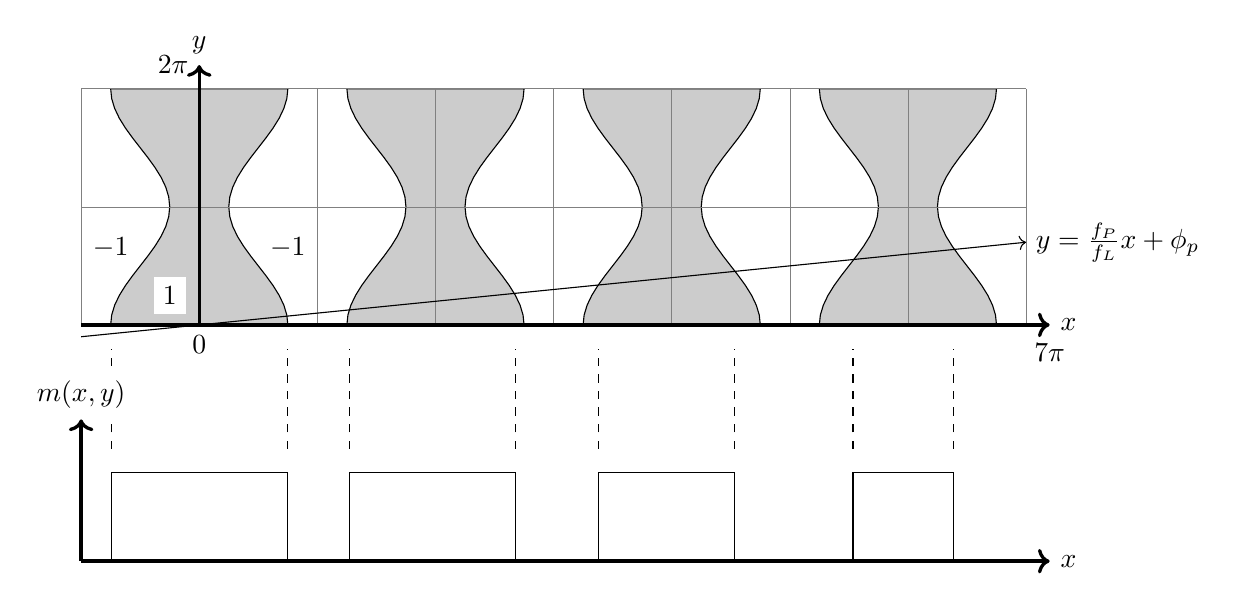
\begin{tikzpicture}[domain=0:1, scale=1.5]
		%% upper half
		% shaded regions
		\drawposregion{0}{0}{2}
		\drawposregion{2}{0}{2}
		\drawposregion{4}{0}{2}
		\drawposregion{6}{0}{2}

		\draw[very thin,color=gray] (-1,0) grid (7,2);
		
		% axis
		\draw[->, very thick] (-1, 0)  
			-- (7.2, 0) node[right] {$x$} node[below=0.1cm] {$7\pi$};
		\draw[->, very thick] (0, 0) node[below]{0}
			-- (0, 2.2) node[above] {$y$} node[left] {$2\pi$};

		% sloped line
		\draw[->] (-1, -0.1) -- (7, 0.7) node[right,fill=white]{$y = \frac{f_P}{f_L} x + \phi_p$};

		% annotations
		\draw (-0.75, +0.65) node[]{$-1$};
		\draw (+0.75, +0.65) node[]{$-1$};
		\draw (-0.25, +0.25) node[fill=white]{$1$};

		%% lower half

		% square wave
		\drawsquare{{-0.5 - 0.25*cos((3.14159 * (0+-0.055)) r) }}
				   {{ 0.5 + 0.25*cos((3.14159 * (0+0.055)) r) }}
				   {-2}{-2+0.75}

		\drawsquare{{1.5 - 0.25*cos((3.14159 * (0.2+-0.055)) r) }}
				   {{2.5 + 0.25*cos((3.14159 * (0.2+0.055)) r) }}
				   {-2}{-2+0.75}

		\drawsquare{{3.5 - 0.25*cos((3.14159 * (0.4+-0.055)) r) }}
				   {{4.5 + 0.25*cos((3.14159 * (0.4+0.055)) r) }}
				   {-2}{-2+0.75}

		\drawsquare{{5.5 - 0.25*cos((3.14159 * (0.6+-0.055)) r) }}
				   {{6.5 + 0.25*cos((3.14159 * (0.6+0.055)) r) }}
				   {-2}{-2+0.75}

		% axis
		\draw[->, very thick] (-1, -2)  
			-- (7.2, -2) node[right] {$x$};
		\draw[->, very thick] (-1, -2)
			-- (-1, -2 + 1.2) node[above,fill=white] {$m(x,y)$};
	\end{tikzpicture}
    \caption{Mapping of Unit Cell to $m(x,y)$ by solution trajectory $y = \frac{f_P}{f_L} x + \phi_p$.}
    \label{fig:double_fourier_mapping}
\end{figure}

If we \textbf{use a small signal approximation} of $v_p << V_L$, we arrive at bounding functions of
\begin{IEEEeqnarray}{rCl}
	x &=& 2 \pi n \pm \arccos (-\frac{v_p}{V_L} \cos y) \quad \forall \, n \in \mathbb{Z} \nonumber\\
	&\approx& 2 \pi n \pm \frac{\pi}{2}\left(1 + M \cos y\right),
\end{IEEEeqnarray}
where $M=\frac{2}{\pi}\frac{v_p}{V_L}$

Double Fourier integral analysis allows us to decompose $m(t)$ into a sum of orthogonal sinusoids as \cite[Chapter~3]{holmes_2003}:
\begin{IEEEeqnarray}{rCl}
	m(t) = \frac{A_{00}}{2} &+& \sum_{n=1}^{\infty} \left[ A_{0n} \cos(ny) + B_{0n} \sin(ny) \right] \nonumber\\
	&+& \sum_{m=1}^{\infty} \left[ A_{m0} \cos(mx) + B_{m0} \sin(mx) \right] \nonumber\\
	&+& \sum_{m=1}^{\infty} \sum_{n\ne0}^{} \left[A_{mn} \cos(mx +ny) + B_{mn} \sin(mx +ny) \right] \\
\end{IEEEeqnarray}

The coefficiencts of the of this problem is presented in past work\cite[Chapter~3]{holmes_2003}:
\begin{IEEEeqnarray}{rCl}
	A_{00} &=& 0 \\
	A_{0n} &=& \begin{cases}
					M \quad & \mathrm{for} \, n=1 \\
					0 \quad & \mathrm{otherwise}
				\end{cases} \\
	A_{mn} &=& \frac{4}{\pi} \frac{1}{m} J_n\left(m \frac{\pi}{2} M\right) \sin\left([m+n]\frac{\pi}{2}\right) \\
	B_{nm} &=& 0
\end{IEEEeqnarray}

To further simplify $A_{mn}$ we can, again, employ a \textbf{small signal approximation} on the Bessel Function of the first kind \eqref{eq:bessel_approx}
\begin{IEEEeqnarray}{rCL}
A_{mn} &=& \frac{4}{\pi} \frac{1}{m} J_n\left(m \frac{\pi}{2} M\right) \sin\left([m+n]\frac{\pi}{2}\right) \nonumber\\
	A_{m0} &\approx& \frac{4}{\pi} \frac{1}{m} \sin\left(m\frac{\pi}{2}\right) \\
	A_{m,\pm1} &\approx& M \sin\left([m\pm n]\frac{\pi}{2}\right) \\
	A_{m,|n|>1} &\approx& 0
\end{IEEEeqnarray}

Ultimately this leaves us with:
\begin{IEEEeqnarray}{rCL}
m(t) &=& \frac{4}{\pi} \sum_{m=1}^{\infty} (-1)^m \frac{1}{2m-1} \cos((2m-1)x) \nonumber\\
	 &+& \frac{v_p}{\pi V_L} \sum_{m} \cos(2mx + y)
\end{IEEEeqnarray}

This spectrum contains the normal harmonics at odd multiples of the grid frequency $f_L$ (as a square wave) but has additional harmonics, all of equal power, at frequencies $2mf_L\pm f_P$. This result is in agreement with \cite{sun_2007}.

\subsection{Mixing Over to DC}

To mix our voltage pertubation over to dc, as in \eqref{eq:mixing_step1}, we convolve the spectrum of the ac voltage and the mixing signal.
\begin{equation}
	\left(\begin{split}
  		M[f] &= \begin{cases}
			(-1)^m \frac{2}{(2m-1)\pi} \quad & \mathrm{for} \, f=(2m+1)f_L \\
			(-1)^m \frac{v_pe^{\pm j \phi_P}}{\pi V_L} \quad & \mathrm{for} \, f= 2mf_L\pm f_P
    	\end{cases}
  	\end{split}\right)
\quad\ast\quad
	\left(\begin{split}
    	V_{ac}[f] &= \begin{cases}
			\frac{V_L}{2} \quad & \mathrm{for} \, f=\pm f_L \\
			\frac{v_p e^{j\phi_P}}{2} \quad & \mathrm{for} \, f=\pm f_P
    	\end{cases}
  	\end{split}\right) \nonumber
\end{equation}

The solution is summarized below\cite{sun_2007}:
\begin{figure}[ht]
	\centering
	\def\arraystretch{2}
	\begin{tabular}{c c c}
	\hline
	f [\si{\hertz}] 		& $V_d[f]$											& Source \\
	\hline
	$(2m+1)f_L\pm f_L$ 		& $(-1)^m \frac{V_L}{(2m+1)\pi}$					& $m[(2m+1)f_L]$, $v_{ac}[\pm f_L]$ \\
	$(2m+1)f_L\pm f_P$ 		& $(-1)^m \frac{v_pe^{\pm j \phi_P}}{(2m+1)\pi}$			& $m[(2m+1)f_L]$, $v_{ac}[\pm f_L]$ \\
	$2mf_L\pm f_P \pm f_L$ 	& $(-1)^m \frac{v_pe^{\pm j \phi_P}}{(2\pi}$	& $m[2mf_L\pm f_P]$, $v_{ac}[\pm f_L]$ \\
	$2mf_L$			 		& $(-1)^m \frac{\cancelToZero{v_p^2}}{2\pi V_L}$					& $m[2mf_L\pm f_P]$, $v_{ac}[\pm f_P]$ \\
	$2mf_L\pm 2f_P$ 		& $(-1)^m \frac{\cancelToZero{v_p^2}e^{\pm j2\phi_P}}{2\pi V_L}$	& $m[2mf_L\pm f_P]$, $v_{ac}[\pm f_P]$ \\
	\end{tabular}
\end{figure}

The \textbf{small signal approximation} allows us to approximate $v_p^2$ as zero.

\subsection{Computing the DC Response}

This analysis \textbf{assumes an linear time invariant DC load} such that the current and voltage relationship can be defined by an admittance as:
\begin{equation}
	i_{dc}[f] = Y_{dc}[f] v_{dc}[f]
\end{equation}

If, for example, we had a constant power load, our relation would instead look like
\begin{equation}
	i_{dc}[nf] = Y_{dc}[f] v_{dc}[f] \frac{P}{2^{n-1}V_T^{n+1}},
\end{equation}
that is, the constant power load would inject a dc current as well as harmonics at integers multiples of the pertubation frequency

\subsection{Mixing Back to AC}
The equation for mixing the currents back to the ac side is
\begin{equation}
	i_{ac}[f] = \sum_k M[k] i_{dc}[f - k].
\end{equation}

We care about $i_{ac}[\pm f_P]$, of which only a few terms are nonzero:
\begin{IEEEeqnarray}{rCl}
	i_{ac}[\pm f_P] &=& M[(2m+1)f_L] i_{dc}[\pm f_P - (2m+1)f_L] \nonumber\\
	&+& M[2mf_L\pm f_P] i_{dc}[\pm f_P - (2mf_L\pm f_P)] \nonumber\\
\end{IEEEeqnarray}

We can check these terms to see if there is a corresponding dc-side current on a linear load
\begin{IEEEeqnarray}{rClr}
\pm f_P - (2m+1)f_L 		&=& (2k+1)f_L \pm f_L \qquad& \text{no solution} \\
\pm f_P - (2m+1)f_L 		&=& (2k+1)f_L \pm f_P \qquad& k = -m-1 \label{eq:ac_side_convolution1}\\
\pm f_P - (2m+1)f_L 		&=& 2kf_L \pm f_P \pm f_L \qquad& k=-m-1,-m \label{eq:ac_side_convolution2}\\
\hline \nonumber\\
\pm f_P - (2mf_L\pm f_P) 	&=& (2k+1)f_L \pm f_L \qquad& k=-m-1,-m \label{eq:ac_side_convolution3}\\
\pm f_P - (2mf_L\pm f_P) 	&=& (2k+1)f_L \pm f_P \qquad& \text{no solution} \\
\pm f_P - (2mf_L\pm f_P) 	&=& 2kf_L \pm f_P \pm f_L \qquad& \text{no solution}
\end{IEEEeqnarray}

\eqref{eq:ac_side_convolution1}, \eqref{eq:ac_side_convolution2}, and \eqref{eq:ac_side_convolution3} will produce terms at $\pm f_P$ on the ac side. 

\eqref{eq:ac_side_convolution1} shows us that we must multiply $M[(2m+1)f_L]$ by $i_{dc}[(2k+1)f_L \pm f_P]$ when $k=-m-1$ to produce:
\begin{IEEEeqnarray}{rCl}
	i_{ac,0} &=& \sum_m M[(2m+1)f_L] \cdot i_{dc}[(2k+1)f_L \pm f_P] \Bigr|_{k=-m-1} \nonumber\\
	&=& \sum_m (-1)^{m}\frac{2}{(2m+1)\pi} \left((-1)^{-m-1} \frac{v_p e^{\pm j \phi_P}}{(-2m-1)\pi} Y_{dc}[(-2m-1)f_L\pm f_P]\right)  \nonumber\\
	&=& \frac{v_p e^{\pm j \phi_P}}{\pi^2} \sum_m \frac{2}{(2m+1)^2} Y_{dc}[-(2m+1)f_L\pm f_P] 
\end{IEEEeqnarray}

Similarly, \eqref{eq:ac_side_convolution2} produces
\begin{IEEEeqnarray}{rCCl}
	i_{ac,1} &=&& \sum_m M[(2m+1)f_L] \cdot i_{dc}[2kf_L \pm f_P \pm f_L] \Bigr|_{k=-m,-m-1} \nonumber\\
	&=&& \sum_m (-1)^{m}\frac{2}{(2m+1)\pi} \left( (-1)^{-m} \frac{v_pe^{\pm j \phi_P}}{2\pi}Y_{dc}[-2mf_L \pm f_P - f_L] \right. \nonumber\\
	&&+& \left. (-1)^{-m-1} \frac{v_pe^{\pm j \phi_P}}{2\pi}Y_{dc}[-2(m+1)f_L \pm f_P + f_L] \right) \nonumber\\
	&=&& 0 %Y_{dc}[-(2m+1)f_L \pm f_P],
\end{IEEEeqnarray}
and \eqref{eq:ac_side_convolution3} produces
\begin{IEEEeqnarray}{rCCl}
	i_{ac,2} &=&& \sum_m M[2mf_L\pm f_P] \cdot i_{dc}[(2k+1)f_L \pm f_L] \Bigr|_{k=-m,-m-1} \nonumber\\
	&=&& \sum_m (-1)^m \frac{v_pe^{\pm j \phi_P}}{\pi V_L} \left((-1)^{-m} \frac{V_L}{(-2m+1)\pi} Y_{dc}[-(2m-1)f_L - f_L] \right. \nonumber\\
	&&+& \left. (-1)^{-m-1} \frac{V_L}{(-2m-1)\pi}Y_{dc}[-(2m+1)f_L + f_L]\right)\nonumber\\
	&=&& \sum_m \frac{v_pe^{\pm j \phi_P}}{\pi^2} \left(\frac{1}{(-2m+1)} + \frac{1}{(2m+1)}\right) Y_{dc}[-2mf_L] \nonumber\\
	&=&& \sum_m \frac{v_pe^{\pm j \phi_P}}{\pi^2} \frac{2}{(1-4m^2)} Y_{dc}[-2mf_L]
\end{IEEEeqnarray}

Combinging the terms, we arrive at
\begin{IEEEeqnarray}{rCl}
	Y_{ac}(s) &=& \frac{4}{\pi^2} \sum_{m} \left( \frac{1}{(2m+1)^2} Y_{dc}(s+j2\pi(2m+1)f_L) - \frac{1}{4m^2-1}Y_{dc}(j4\pi m f_L)\right).
\end{IEEEeqnarray}

\subsection{Resistive Load}

Consider a resistor with resistance $R$ and admittance $G = 1/R$. The ac-side admittance (and impedance) can be found using \eqref{eq:infinite_sum1} and \eqref{eq:infinite_sum2}:

\begin{IEEEeqnarray}{rCl}
	Y_{ac}(s) &=& \frac{4}{\pi^2} \sum_{m} \left( \frac{1}{(2m+1)^2} G - \frac{1}{4m^2-1}G\right) \nonumber\\
	&=& \frac{4G}{\pi}  \sum_{m} \left( \frac{1}{(2m+1)^2} - \frac{1}{4m^2-1}\right) \nonumber\\
	&=& \frac{4G}{\pi}  \left(\frac{\pi^2}{4} - 0\right) \nonumber\\
	&=& G
\end{IEEEeqnarray}

\subsection{Connection to Envelope Impedance}

Envelope Impedance is the case where rather than one injected pertubation, the amplitude of the line voltage is modulated.
Amplitude modulation may be written as the sum of two sidebands as follows:

\begin{IEEEeqnarray}{rCl}
	y_{AM}(t) &=& (1 + m\cos(2\pi f_{AM}t+\phi)) A \sin(2\pi f_Lt) \nonumber\\
	&=& A \sin(2\pi f_L t) + \frac{1}{2}Am\left(\sin(2\pi(f_L+f_{AM})t+\phi) - \sin(2\pi(f_L-f_{AM})t-\phi))\right)
\end{IEEEeqnarray}

An important term in the mixing signal used in small signal impedance modeling is the result of conduction angle modulation.
That is, cycle to cycle variations in 

%%%%%%%%%%%%%%%%%%%%%%%%%%%%%%%%%%%%%%%%%%%%%%%%%%%%%%%%%%%%%%%%%%%%%%%%%%%%%%%
%%%%%%%%%%%%%%%%%%%%%%%%%%%%%%%% Conclusion %%%%%%%%%%%%%%%%%%%%%%%%%%%%%%%%%%%
%%%%%%%%%%%%%%%%%%%%%%%%%%%%%%%%%%%%%%%%%%%%%%%%%%%%%%%%%%%%%%%%%%%%%%%%%%%%%%%
\section{Conclusion}

% \begin{figure}[htbp]
%     \center
%     \includegraphics[width=0.5\linewidth]{figs/cpl_fourier_rect.png}
%     \caption{Fourier and small signal approximation to constant power load current.}
%     \label{fig:results}
% \end{figure}


%%%%%%%%%%%%%%%%%%%%%%%%%%%%%%%%%%%%%%%%%%%%%%%%%%%%%%%%%%%%%%%%%%%%%%%%%%%%%%%
%%%%%%%%%%%%%%%%%%%%%%%%%%%%%%%%% Appendix %%%%%%%%%%%%%%%%%%%%%%%%%%%%%%%%%%%%
%%%%%%%%%%%%%%%%%%%%%%%%%%%%%%%%%%%%%%%%%%%%%%%%%%%%%%%%%%%%%%%%%%%%%%%%%%%%%%%

\setcounter{section}{0}
\renewcommand\thesection{\Alph{section}}
\renewcommand\theequation{\Alph{section}.\arabic{equation}}
\section*{Appendix}

\setcounter{equation}{0}
\section{Arithmetic Series}

First, the sum of inverse squares (Basel problem) and also the sum of even squares 
\begin{IEEEeqnarray}{rCl}
	\sum_{m=1}^{\infty} \frac{1}{m^2} &=& \frac{\pi^2}{6} \\
	\sum_{m=2,4,\ldots}^{\infty} \frac{1}{m^2} &=& \sum_{m=1}^{\infty} \frac{1}{(2m)^2} = \frac{1}{4}\frac{\pi^2}{6}
\end{IEEEeqnarray}

Now, a helpful infinite sum
\begin{IEEEeqnarray}{rCl}
	\sum_{m} \frac{1}{(2m+1)^2} &=& 2\sum_{k=1,3,\ldots}^{\infty} \frac{1}{k^2} \nonumber\\
	&=& 2\left(\sum_{m=1}^{\infty} \frac{1}{m^2} - \sum_{m=2,4,\ldots}^{\infty} \frac{1}{m^2}\right) \nonumber\\
	&=& 2\left(\frac{\pi^2}{6} - \frac{1}{4}\frac{\pi^2}{6}\right) \nonumber\\
	&=& \frac{\pi^2}{4}. \label{eq:infinite_sum1}
\end{IEEEeqnarray}

For another helpful infinite sum, we start with the positive half finite sum
\begin{IEEEeqnarray}{rCl}
	\sum_{m=1}^{n}\frac{1}{4m^2-1} &=& \sum_{m=1}^{n}\frac{1}{2} \left(\frac{1}{2m-1}-\frac{1}{2m+1}\right) \nonumber\\
	&=& \frac{1}{2}\left(\sum_{m=1}^{n}\left(\frac{1}{2m-1}\right)-\sum_{m=1}^{n}\left(\frac{1}{2m+1}\right)\right) \nonumber\\
	&=& \frac{1}{2}\left(1 + \sum_{m=2}^{n}\left(\frac{1}{2m-1}\right) - \sum_{m=1}^{n-1}\left(\frac{1}{2m+1}\right) - \frac{1}{2n+1} \right)\nonumber\\
	&=& \frac{1}{2}\left(1 + \cancelRed{\sum_{p=m-1=1}^{n-1}\left(\frac{1}{2(p+1)-1}\right)} - \cancelRed{\sum_{m=1}^{n-1}\left(\frac{1}{2m+1}\right)} - \frac{1}{2n+1} \right)\nonumber\\
	&=& \frac{1}{2}\left(1 - \frac{1}{2n+1}\right).
\end{IEEEeqnarray}

We can find the positive half infinite sum by taking the limit as $n\rightarrow\infty$
\begin{IEEEeqnarray}{rCl}
	\sum_{m=1}^{\infty}\frac{1}{4m^2-1} &=& \lim_{n\rightarrow\infty} \frac{1}{2}\left(1-\frac{1}{2n+1}\right) \nonumber\\
	&=& \frac{1}{2}
\end{IEEEeqnarray}

Finally, we can find the infinite sum:
\begin{IEEEeqnarray}{rCl}
	\sum_{m} \frac{1}{4m^2-1} &=& -1 + 2\sum_{m=1}^{\infty}\frac{1}{4m^2-1} \nonumber\\
	&=& -1 + 2 \frac{1}{2} \nonumber\\
	&=& 0 \label{eq:infinite_sum2}
\end{IEEEeqnarray}

\setcounter{equation}{0}
\section{Bessel Function of the First Kind}

The Bessel Function of the first kind has a series representaion for integer values of $n$ \cite{weisstein_bessel}, shown below for reference:
\begin{IEEEeqnarray}{rCl}
	J_n(x) &=& \sum_{k=0}^{\infty} \frac{(-1)^k}{k!(|n|+k)!} \left(\frac{x}{2}\right)^{|n|+2k}
\end{IEEEeqnarray}

Let $x << 1$, we may then approximate the Bessel Function by eliminating all the terms of $k>0$ leaving us with
\begin{IEEEeqnarray}{rCl}
	J_n(x) &=& \frac{1}{|n|!} \left(\frac{x}{2}\right)^{|n|}
\end{IEEEeqnarray}

Taking this one step further, we can approximate all Bessel Function with $n>1$ as zero, resulting in
\begin{IEEEeqnarray}{rCl}
	J_0(x<<1) &\approx& 1 \\
	J_{\pm1}(x<<1) &\approx& \frac{x}{2} \\
	J_{n>1}(x<<1) &\approx& 0 \label{eq:bessel_approx}
\end{IEEEeqnarray}



% \subsection{Pictures}

% \begin{figure}[htbp]
%     \center
%     \includegraphics[scale=0.06]{img/photo.jpg}
%     \caption{Sydney, NSW}
% \end{figure}

% \subsection{Citation}

% This is a citation\cite{Eg}.

\newpage

% ------------------------------------------------------------------------------
% Reference and Cited Works
% ------------------------------------------------------------------------------

\bibliographystyle{IEEEtran}
\begin{thebibliography}{1}

% \bibitem{leonard_2014}
% J.\@ P.\@ Leonard, ``Nonlinear Modeling Of Dc Constant Power Loads With Frequency Domain Volterra Kernels,''Florida State University, 2014.

\bibitem{sun_2007}
J. Sun and K. J. Karimi. ``Small-Signal Input Impedance Modeling of Line-Frequency Rectifiers,'' \emph{IEEE. Trans. on Aerospace and Electronics Systems}, Vol. 44, Number 4, October, 2008.

\bibitem{bing_2011}
Z. Bing and J. Sun. ``Frequency-Domain Modeling of Multipulse Converters by Double-Fourier Series Method,'' \emph{IEEE. Trans. on Power Electronics}, Vol. 26, Number 12, December, 2011.

\bibitem{holmes_2003}
D. G. Holmes, ``Pulse width modulation for power converters: principles and practice,'' IEEE Press, 2003.


\bibitem{weisstein_bessel}
 E. W. Weisstein, ``''Bessel Function of the First Kind,'' MathWorld--A Wolfram Web Resource. https://mathworld.wolfram.com/BesselFunctionoftheFirstKind.html 



\end{thebibliography}
% ------------------------------------------------------------------------------

\end{document}